

\documentclass[12pt]{article} % format du document
\usepackage[utf8]{inputenc} % type d'encodage utf8 unix, le plus worlwide
% \usepackage[round]{natbib} % package de format biblio
\usepackage[T1]{fontenc} % police d'encodage, OT1 moins de caractère que T1 (qui contient les caractères spéciaux)
\usepackage[english,francais]{babel} % package de langue
\usepackage{amsmath} % pour écrire les formules maths et améliorer la sortie
\usepackage{amssymb} % symboles additionnels pour amsmath
\usepackage{mathrsfs} % des symboles additionnels de physique (entre autre)
\usepackage[pdftex]{graphicx} % package pour les graphiques, version avancée
\usepackage[hmargin=2.5cm, vmargin=2cm]{geometry} % marges
\usepackage{setspace} % interlignes
\usepackage{fancyhdr} % customisation des hauts et bas de page
\usepackage[svgnames, table]{xcolor} % contrôle des couleurs avancé
\usepackage[unicode=true]{hyperref} % pour les liens et customisation de ceux-ci
\usepackage{verbatim}
\usepackage{listings} % pour du code, certains langages prédéfini, sortie simple
\usepackage{lastpage} % pour récupérer la dernière page
\usepackage{times} % police d'écriture
\usepackage{titlesec} % formatage des titres
\usepackage{framed}
%\overfullrule=2cm

\titlespacing{\paragraph}{0em}{1em}{1em} % pas de tabulation pour subsubsection, 1.5em espace au dessus, 0.5em en dessous

%%%%%%%%%%% Configuration couleurs & auteur du pdf %%%%%%%%%%%%%%%%%%%%%%%%%%%%%%%%%%%%%%%%%%
\hypersetup{breaklinks=true,
            pdfauthor={Bastien Delseny},
            pdftitle={Triangle de Pascal},
            colorlinks=true,
            citecolor=DarkGreen,
            urlcolor=blue,
            linkcolor=DarkRed,
            pdfborder={0 0 0}}
%%%%%%%%%%%%%%%%%%%%%%%%%%%%%%%%%%%%%%%%%%%%%%%%%%%%

%----------- Configuration de listings --------------%
%breaklines => retours à la ligne
%postbreak => configuration du retour à la ligne
\lstset{
    frame=single,
    breaklines=true,
    postbreak=\raisebox{0ex}[0ex][0ex]{\ensuremath{\color{red}\hookrightarrow\space}}
}

%----------------- VERBATIM ---------------------%
\makeatletter
\newcommand{\verbatimfont}[1]{\def\verbatim@font{#1}}%
\makeatother
\verbatimfont{\color{DarkGreen}\sffamily}

% ---------------- URLS ----------------------------------%
\urlstyle{same}  % don't use monospace font for urls
\newcommand{\HRule}{\rule{\linewidth}{0.5mm}} %Hrule fait des lignes horizontales de 0.5mm d'épaisseur

%%%%%%%%%%%%% On met une ligne en haut et bas de page %%%%%%%%%%%%%%%%%%%%%%
\renewcommand{\headrulewidth}{0.1pt}
%\renewcommand{\footrulewidth}{0.1pt}
%%%%%%%%%%%%%%%%%%%%%%%%%%%%%%%%%%%%%

%%%%%%%%%%%%% On crée une commande pour faire des saut de paragraphe réglables 0em par défault %%%%%%%%%%%%%%%%%%%%%
\newcommand{\PAR}[1][0em]{\setlength{\parskip}{#1}\par}
%%%%%%%%%%%%%%%%%%%%%%%%%%%%%%%%%%%%%%%%%%%%%%%%%%%%%%%%%

%%%%%%%%%%%%%%%%%%%%%%%%%%%%%%%%%%%%%%%%%%%%%%%%%%%%%%%%%%%%%%%%%%%%%%%%%%%%%%%%%
%							DOCUMENT											%
%%%%%%%%%%%%%%%%%%%%%%%%%%%%%%%%%%%%%%%%%%%%%%%%%%%%%%%%%%%%%%%%%%%%%%%%%%%%%%%%%
\begin{document}

	%-------------------------------------------------------------------------------%
	%							Page de garde										%
	%-------------------------------------------------------------------------------%
	%%%%%%%%%%%%%%%%%%%%%%%%%%%%%%%%%%%%%%%%%%%%%%%%%%%%%%%%%%%%%%%%%%%%%%%%%%%%%%%%%
%							Page de garde										%
%%%%%%%%%%%%%%%%%%%%%%%%%%%%%%%%%%%%%%%%%%%%%%%%%%%%%%%%%%%%%%%%%%%%%%%%%%%%%%%%%
\begin{titlepage}
  \begin{center}
	
	% Logo UGA
	
      \begin{flushleft} 
       
\includegraphics[width=0.3\textwidth]{./images/logo-uga}~\\
       {\small Université Grenoble Alpes}
      \end{flushleft}
    
    
    \vfill

    % Titre
    \HRule \\[0.4cm]
    { \huge \bfseries Triangle de Pascal\\[.4em]}
    \HRule\\[4em]
    
      % Image de garde
	\begin{centering}
		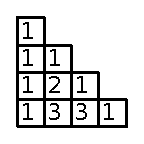
\includegraphics[width=0.4\textwidth]{./images/triangle}
	\end{centering}\\[4em]
	
    % Auteur
	\large{Bastien Delseny}\\
   \vfill
    
    % Bas de page
    \rule{\linewidth}{0.1mm} \\[0.3cm]
    
    {\footnotesize M2 - CCI}\\[0.3cm]
    
    
    {\large 11 Janvier 2015 — 11 Juin 2015} \PAR

  \end{center}
\end{titlepage}


	%%%%%%%%%%%%%%%%%%%%%%%%%%%%%%%%%%%%%%%%%%%%%%%%%%%%%%%%%%%%%%%%%%%%%%%%%%%%%%%%%
	%						Table des matières										%
	%%%%%%%%%%%%%%%%%%%%%%%%%%%%%%%%%%%%%%%%%%%%%%%%%%%%%%%%%%%%%%%%%%%%%%%%%%%%%%%%%
	\normalsize
	\clearpage
	\pagestyle{empty}
	\renewcommand{\contentsname}{Table des matières}
	\setstretch{2}
	\vspace*{\fill} \tableofcontents \vfill

	%%%%%%%%%%%%%%%%%%%%%%%%%%%%%%%%%%%%%%%%%%%%%%%%%%%%%%%%%%%%%%%%%%%%%%%%%%%%%%%%%
	%									RAPPORT										%
	%%%%%%%%%%%%%%%%%%%%%%%%%%%%%%%%%%%%%%%%%%%%%%%%%%%%%%%%%%%%%%%%%%%%%%%%%%%%%%%%%
	\clearpage
	%	\pagestyle{fancy}
	%		\lhead{\leftmark}
	%		\chead{ }
	%		\rhead{Bastien Delseny}
	%		\lfoot{\textit{Gestion multifonctionnelle d'une for\^{e}t en univers risqu\'e}}
	%		\cfoot{}
	%		\rfoot{\thepage/\pageref*{ArabePage}}
		\pagestyle{fancy}
			\lhead{}
			\chead{\rightmark}
			\rhead{}
			\lfoot{}
			\cfoot{}
			\rfoot{\thepage/\pageref*{ArabePage}}
	%%%%%%%%%%%%%%%%%%%%%%%%%%%%%%%%%%%%%%%%%%%%%%%%%%%%%%%%%%%%%%%%%%%%%%%%%%%%%%%%%
	%						TEXTE DU RAPPORT										%
	%%%%%%%%%%%%%%%%%%%%%%%%%%%%%%%%%%%%%%%%%%%%%%%%%%%%%%%%%%%%%%%%%%%%%%%%%%%%%%%%%
	\clearpage
	\setstretch{1.5}
	\setcounter{page}{1}
	\section{Compilation et génération du fichier exécutable}

\subsection{Compilation de triangle}
L'exécution du programme triangle permet d'obtenir les instructions en PostScript pour la construction d'un triangle de Pascal de taille de police et de nombre de lignes voulu.
Pour exécuter ce programme il suffit d'exécuter la commande \verb|>./triangle 12 4| ce qui donnera les instructions en PostScirpt pour créer un triangle de Pascal de taille de police 12 et de 4 lignes (code \ref{triangle}).
\begin{lstlisting}[language=PostScript, label=triangle, caption=./triangle 12 4]
newpath 24 245 moveto 38 245 lineto 38 260 lineto stroke newpath 24 245 moveto 24 260 lineto 38 260 lineto stroke /Courier findfont 12 scalefont setfont newpath 25 248 moveto (1) show 
newpath 24 230 moveto 38 230 lineto 38 245 lineto stroke newpath 24 230 moveto 24 245 lineto 38 245 lineto stroke /Courier findfont 12 scalefont setfont newpath 25 233 moveto (1) show 
etc ...
\end{lstlisting}

\subsection{Redirection de la sortie standard}
\label{sec:sortie}

La commande \verb|>./triangle 12 4 > triangle_pascal_12_4.ps| permet de rediriger la sortie standard vers le fichier \verb|triangle_pascal_12_4.ps| qui contient le code PostScript \ref{triangle}.
À l'aide de la commande \verb|> cat triangle_pascal_12_4.ps| on affiche dans le terminal le code PostScript (code \ref{triangle}) enregistré dans \verb|triangle_pascal_12_4.ps|.
À l'aide de la commande \verb|>gv triangle_pascal_12_4.ps| l'interprète de langage PostScript nous permet d'observer la figure \ref{fig:triangle_12_4}.

\begin{figure}[!h]
\begin{centering}
	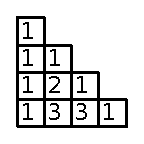
\includegraphics[width=0.5\textwidth]{./images/triangle}
	\caption{Triangle de Pascal de taille de police 12 de 4 lignes.}
	\label{fig:triangle_12_4}
	\end{centering}
\end{figure}

\subsection{Redirection de l'entrée standard}
L'exécution de la commande \verb|> tr "bc" "BC" < Makefile| permet de mettre en majuscule les lettres c et b du fichier \verb|Makefile|. 

\subsection{Tube et chaînage de commandes}
\label{sec:tube}
Lorsque l'on exécute la commande \verb|> date > d| on redirige la sortie de l'exécution de la commande \verb|> date| vers le fichier \verb|d|.
L'exécution de la commande \verb|> tr ":" "_" < d| permet de récupérer ce que contient le fichier \verb|d| afin de remplacer les \verb|:| par des \verb|_|.
À l'aide de l'utilisation d'un tube de redirection il est possible d'effectuer la même manoeuvre sans passer par un fichier intermédiaire et afficher le résultat directement dans le terminal.
C'est ce que permet de faire la commande \verb!date \| tr ":" "_"!.

Ainsi en utilisant les commandes \ref{pipeBash} on obtient la même figure \ref{fig:triangle_12_4} qu'en effectuant les démarche de la section \ref{sec:sortie} qui sera affichée par un interpréteur de PostScript.

\begin{lstlisting}[language=bash, label=pipeBash, caption=Tubes de redirection]
> ./triangle 12 4 | gs -sDEVICE=x11 -q
> ./triangle_12_4 | gv -
\end{lstlisting}














	\section{Lancement de l'interprète PostScript par exec}

Les exécutables des commandes \verb!gv! et \verb!gs! se trouvent dans les répertoire \verb!/usr/bin/gv! et \verb!/usr/bin/gs!, chemin qu'il a été possible de trouver grâce à la commande \verb!which!.
Ainsi exécuter la commande \verb!>/usr/bin/gv triangle.ps! revient au même que d'exécuter la commande \verb!>gv triangle.ps!.

Afin d'exécuter directement l'interpreteur de PostScript lors de l'exécution du programme il faut modifier le code source de \verb!affiche_triangle!.
Il faudra commencer par initialiser deux variables. Un texte contenant le chemin de la commande de l'interpréteur PostScript à utiliser. Ainsi qu'un tableau de texte contenant la commande ainsi que ces arguments. Le code nécessaire pour l'interpréteur \verb!gv! et celui pour \verb!gs! est ici : \ref{lst:variables_q2}.

\begin{lstlisting}[language=C, label={lst:variables_q2}, caption=Initialisation des variables pour exec de gv et gs]
/*	Arguments pour gv	*/
char nomGV [] = "/usr/bin/gv";
char *argumentsGV [] = {"/usr/bin/gv", "triangle.ps", NULL};

/*  Arguments pour gs	*/
char nomGS [] = "/usr/bin/gs";
char *argumentsGS [] = {"/usr/bin/gs", "-q", "-sDEVICE=x11", "triangle.ps", NULL};
\end{lstlisting}

Ensuite il faudra ajouter la commande \verb!execve(...)! correspondante à l'interprète choisi à la fin du \verb!main()! (code \ref{lst:code_exec})

\begin{lstlisting}[language=C, label={lst:code_exec}, caption=Appel de la fonction execve() pour gv et gs]
/*  Execution de gv	*/
execve(nomGV, argumentsGV, envp);

/*  Execution de gs	*/
execve(nomGS, argumentsGS, envp);
\end{lstlisting}

Puis il faut recompiler le code avec \verb!>make!. Il suffira d'exécuter le programme à l'aide de la commande \verb!>./triangle 12 4 > triangle.ps! pour obtenir le même résultat que pour la section \ref{sec:tube}. On peut en plus rediriger la sortie standard d'erreur dans un fichier à l'aide de l'option \verb! 2> fichier.log! comme suit \verb!>./triangle 12 4 > triangle.ps 2> triangle.log!.


	\section{Lancement de gs par fork et exec}
\subsection{Vérification de la taille de police et du nombre de lignes}

Afin de vérifier si la taille de la police et si le nombre de ligne sont correctes on peut ajouter le code suivant \ref{lst:verif} dans le code source de \verb!affiche_triangle.c!

\begin{lstlisting}[language=C, label={lst:verif}, caption={Vérification de la taille de police comprise entre 8 et 24, et du nombre de lignes comprit entre 1 et 40.}]
  if(taille_police < 8 || taille_police > 24){
	  fprintf(stderr, "Taille de police incorrecte, valeur entre 8 et 24 attendue\n");
	  exit(1);
  }
  if(nb_lignes < 1 || nb_lignes > MAX_LIGNES){ // MAX_LIGNES = 40
	  fprintf(stderr, "Nombre de lignes incorrecte, valeur entre 1 et %d attendue\n", MAX_LIGNES);
	  exit(1);
  }
\end{lstlisting}

\subsection{Une histoire de père et de fils}
La fonction C \verb!fork()! permet de créer un fils. 
Il faut commencer par initialiser deux variables dans \verb!affiche_triangle.c!.
Une variable qui permettra de récupérer le pid du fils grâce à la commande \verb!pid_t p;!.
Il faut aussi une variable qui permettra de récupérer le code de retour, code d'erreur ou de réussite de la fin d'exécution du fils, grâce à la commande \verb!int retour;!.
Afin que le processus fils exécute \verb!gv! ou \verb!gs! il faut procéder comme indiquer dans le code \ref{lst:pereFils}.

\begin{lstlisting}[language=C, label={lst:pereFils}, caption={Création d'un fils qui execute la fonction execve permettant la lecture du fichier PostScript par un interpréteur de PostScript.}]
/* Generation des triangles par le pere */
sortie = "stdout";
taille_triangle = nb_lignes;
postscript_triangle (taille_police);
sleep (3);

/* Creation d'un processus fils */
p = fork();

/* Verification de la creation d'un fils a l'aide de la commande fork */
if(p < 0) {
	fprintf(stderr, "Luke (fils) n'a pas pu etre creer par fork\nVador (pere) est triste\n");
	exit(1);
}

/* Fils creer  plus qu'a attendre qu'il affiche les triangles*/
if(p != 0){
	/* Attendre la terminaison du fils */
	wait(&retour);
	fprintf(stderr, "Generation et affichage du triangle de Pascal termine\n");
} else {	
	/* Execution de l'interpreteur de PostScript */
	execve(nomGV, argumentsGV, envp);
	//execve(nomGS, argumentsGS, envp);
}
\end{lstlisting}

	\section{Génération du PostScript dans un fichier.}

Après avoir généré le PostScript du triangle dans \verb!triangle.ps! il est possible de connaître la taille de ce fichier PostScript. 
Pour cela il suffit d'effectuer la commande \verb!ls -l triangle.ps! dans le terminal.
On observe que la taille du fichier est de $1,9ko$, appelons $T1$ cette taille.

\subsection{Un problème de taille}

Après avoir supprimé le fichier de $1,9ko$ \verb!triangle.ps! et modifié le code de la procédure main pour affecter la sortie à un fichier \verb!triangle.ps! il faut compiler le code et exécuter le programme.
À la fin de l'exécution il y a un nouveau fichier \verb!triangle.ps!.
Ce fichier fait une taille $T2$ de $185o$. 
La taille de ce nouveau fichier $T2$ est donc largement inférieure à la taille du fichier précédent $T1$.
Lorsque l'on ouvre \verb!triangle.ps! avec un interpréteur de PostScript on se rend compte qu'un seul triangle a été créé.

\subsection{Il nous manque des cases}
\label{sub:cases}

La ligne $66$ de la fonction \verb!boite_chiffre()! du code \verb!boite_chiffre.c! permet de définir les options d'écriture dans le fichier de sortie.
On remarque que le code est le suivant : \verb!fsortie = fopen(sortie, ``w'')!.
L'option \verb!w! permet de créer un nouveau fichier, en supprimant celui existant, et d'écrire dans ce fichier.
Or dans le code \verb!affiche_triangle.c! on observe que la fonction \verb!postscript_triangle()! fait appelle à une boucle sur la fonction \verb!boite_chiffre()!.
Donc à chaque appel de \verb!boite_chiffre()! un nouveau fichier va être créé et une seule boite sera dessinée.
Pour palier à ce problème il nous faut changer l'option \verb!w! de la fonction \verb!fopen()! par l'option \verb!a! qui permet de continuer l'écriture dans le fichier existant si celui-ci existe, sinon de créer le fichier.

\subsection{Un problème de superposition}

Maintenant un nouveau problème fait face.
Lorsque nous lançons plusieurs fois l'exécution du programme les triangles se superposent.
Ce qui rend à la fois la présentation des triangles illisibles et la taille des fichiers exponentielle.
Il faut donc qu'au début de l'exécution du programme un nouveau fichier soit créé afin de ne pas ré-écrire à la suite d'un fichier existant.
Pour ce faire il faut modifier le code de la fonction \verb!postscript_triangle()! du code \verb!affiche_triangle.c!.
Il faut en début de cette fonction initialiser un fichier si la sortie n'est pas la sortie standard.
On rajoute alors le code \ref{lst:sortiePremiere} en début de la fonction \verb!postscript_triangle()!

\begin{lstlisting}[language=C, label={lst:sortiePremiere}, caption={Initialisation du fichier de sortie.}]
if( strcmp(sortie, ``stdout'') != 0 ) {
  fopen(sortie, ``w'');
}
\end{lstlisting}

On remarque que suite à cette modification la taille du fichier sera la même en mettant la sortie vers un fichier dans le code source du programme ou en redirigeant la sortie standard vers un fichier.
Ainsi à la fin de ces modification $T1=T2$.


	\section{Création d'un tube entre triangle et gs}

Le but ici est que le processus père créer un tube et créer deux fils qui intéragissent à l'aide de ce tube.
Ainsi on commence par créer un tube de redirection à l'aide de la commande \verb!pipe()!.
Une fois le tube créé, on crée un processus fils qui va générer le PostScript de triangle vers l'entrée du tube.
Ainsi la sortie standard est redirigée vers l'entrée du tube de redirection.
On termine le processus fils et on créer un nouveau processus fils.\\
On redirige l'entrée standard, qui sera donc celle du nouveau fils, vers la sortie du tube de redirection.
Le processus fils lance alors l'interprète de PostScript.\\
Une fois que l'interpréteur de PostScript est terminé, on termine le processus fils puis on ferme le tube de redirection.\\
L'ensemble du code est détaillé ici : \ref{lst:tubeq5}.

\begin{lstlisting}[language=C, label={lst:tubeq5}, caption={Utilisation d'un tube dans la fonction main.}]
int main(int argc, char *argv[], char *envp[])
{
  /* Initialisation des variables */
  unsigned int taille_police, nb_lignes;
  char nom_executable[200];
  pid_t p_gauche, p_droit;
  int retour_gauche, retour_droit;
  int tube[2];

  lire_args(argc,argv,3,message_usage, 
        "%s",nom_executable,"",
        "%d",&taille_police,"taille_de_police_incorrecte",
        "%d",&nb_lignes,"nombre de lignes incorrect");

  /* Verification des valeurs */
  /* de taille_police [8,24] et nb_lignes [1,MAX_LIGNES]  */
  if(taille_police < 8 || taille_police > 24){
          fprintf(stderr, "Taille de police incorrecte, valeur entre 8 et 24 attendue\n");
          exit(1);
  }
  if(nb_lignes < 1 || nb_lignes > MAX_LIGNES){
          fprintf(stderr, "Nombre de lignes incorrecte, valeur entre 1 et %d attendue\n", MAX_LIGNES);
          exit(1);
  }
    
        /* Creation d'un tube */
        pipe(tube);

        /* Fils gauche */
        p_gauche = fork();
        
        if(p_gauche < 0) { // erreur
                fprintf(stderr, "Le fils n'a pas pu etre cree\n");
        }

		/* Le fils gauche genere le PostScript,
			envoie la sortie standard vers l'entree du tube */
        if(p_gauche == 0){
                close(tube[0]); // fermeture de la sortie du tube
                dup2(tube[1],1);
                sortie = "stdout";
                taille_triangle = nb_lignes;
                postscript_triangle (taille_police);
                sleep (3);
                close(tube[1]);
                exit(0);
                
        }

		p_droit = fork();
        if(p_droit < 0) { // erreur
                fprintf(stderr, "Le fils n'a pas pu etre cree\n");
        }
		
		/* Le fils droit recupere la sortie du tube,
			ouvre l'interprete de PostScript */
        if(p_droit == 0){
                close(tube[1]); // On ferme la sortie du tube
                dup2(tube[0],0);
                execve(nomGV, argumentsGV, envp);
                close(tube[0]);
                exit(0);
        }

        /* fermeture des tubes du pere */    
        close(tube[0]);
        close(tube[1]);

        /* Attente de la fin des fils */
        waitpid(p_gauche, &retour_gauche, 0);
        waitpid(p_droit, &retour_droit, 0);
        
        fprintf(stderr, "Generation et affichage du triangle de Pascal termine\n");
        
        
  return 0;
}
\end{lstlisting}

	%%%%%%%%%%%%%%%%%%%%%%%%%%%%%%%%%%%%%%%%%%%%%%%%%%%%%%%%%%%%%%%%%%%%%%%%%%%%%%%%%
	%							BIBLIOGRAPHIE										%
	%%%%%%%%%%%%%%%%%%%%%%%%%%%%%%%%%%%%%%%%%%%%%%%%%%%%%%%%%%%%%%%%%%%%%%%%%%%%%%%%%
	\normalsize
	% \addcontentsline{toc}{section}{R\'ef\'erences bibliographiques}
	% \bibliographystyle{plainnat}
	% \setstretch{1}
	% \bibliography{Revue}
	%\renewcommand{\listfigurename}{Images et figures}
	%\listoffigures
	\label{ArabePage}

\end{document}
%test
